\id{МРНТИ 65.63.03}{https://doi.org/10.58805/kazutb.v.2.27-1004}
\vspace{0.5em}
\begin{articleheader}
\sectionwithauthors{N. Alzhaxina, A. Dalabayev, I. Aubakirova, М. Mantay}{OPTIMIZATION OF THE FORMULATION OF A CURD PRODUCT WITH THE ADDITION OF PUMPKIN CRYOPOWDER}

{\bfseries
N. Alzhaxina\alink{https://orcid.org/0000-0001-7855-0940}\textsuperscript{\envelope },
A. Dalabayev\alink{https://orcid.org/0000-0001-7811-0697},
I. Aubakirova\alink{https://orcid.org/0009-0008-6306-4630},
М. Mantay\alink{https://orcid.org/0000-0003-0822-0932}
}
\end{articleheader}

\begin{affiliation}
Astana branch «Kazakh research institute of processing and food industry» LTD, Astana, Kazakhstan

\raggedright \textsuperscript{\envelope }Corresponding author: alzhaxina@inbox.ru
\end{affiliation}

Formulations of structured dairy products that demonstrate good
organoleptic properties are considered the most promising in terms of
meeting consumer demands, increasing market share, and enhancing the
competitiveness of domestic dairy production. The selection of dairy
bases (low-fat curd, pumpkin cryopowder, and cream), which possess
diverse structural-mechanical characteristics and
functional-tech\-nological properties, is scientifically justified and
aimed at developing a range of structured dairy products containing
functional food components. Viscosity was chosen as the target function
for optimization, as it is a key indicator characterizing the
consistency and structure of viscous products, such as the curd-based
product being developed. An analysis of the response surface revealed
that the optimal viscosity zone for the curd product is achieved when
the mass fraction of curd is 89.6\%, the mass fraction of cryopowder is
5.4\%, and the fat content in the cream is 31.3\%. The characteristic
viscosity for curd products ranges from 1400 to 2500 mPa·s. The analysis
of prediction error distribution for viscosity values yielded
satisfactory results: a significant portion of the data points remained
close to the trendline, confirming the adequacy of the model. This
indicates the formation of a product structure in which the fermented
protein coagulate plays a key role. Therefore, the viscosity,
consistency, and consumer properties of the final product largely depend
on its concentration.

{\bfseries Keywords:} optimization, formulation, curd product, pumpkin
cryopowder, low-fat curd, cream, visco\-sity, Box--Behnken three-level
design.

\begin{articleheader}
{\bfseries АСҚАБАҚ КРИОҰНТАҒЫ ҚОСЫЛҒАН СҮЗБЕ ӨНІМІНІҢ РЕЦЕПТУРАСЫН ОҢТАЙЛАНДЫРУ}

{\bfseries
Н.E. Альжаксина\textsuperscript{\envelope },
А.Б. Далабаев,
И.Е. Аубакирова,
М.С. Мантай
}
\end{articleheader}

\begin{affiliation}
Астана филиалы ЖШС «Қазақ қайта өңдеу және тағам өнеркәсіптері ғылыми-зерттеу институты, Астана, Қазақстан,

е-mail: alzhaxina@inbox.ru
\end{affiliation}

Жақсы органолептикалық сипаттамалары бар құрылымдық сүт өнімдерінің
рецептураларын тұтыну талаптарын қанағаттандыру, нарықтық үлесті арттыру
және отандық сүт өнімдерінің бәсекеге қабілеттілігін арттыру үшін ең
перспективалы деп санауға болады. Әр түрлі құрылымдық-механикалық
сипаттамалары мен функционалдық-технологиялық қасиеттері бар сүт
негіздерін (майсыз сүзбе, асқабақ криоұнтағы, кілегей) таңдау ғылыми
негізделген және функционалды тағамдық компоненттері бар құрылымдық сүт
өнімдерінің желісін жасауға бағытталған. Оңтайландыруға тиісті мақсатты
функция ретінде тұтқыр өнімдердің консистенциясы мен құрылымын
сипаттайтын көрсеткіш ретінде, сүт өнімін дамытудағы тұтқырлық таңдалды.
Алынған жауап бетінің мінез-құлқын талдау көрсеткендей, тұтқырлықтың
оңтайлы аймағы, ол сүзбенің массалық үлесі 89,6\%, криоұнтақтың массалық
үлесі - 5,4\% және кілегейдегі майдың массалық үлесі - 31,3\% болғанда
жетеді. Сүзбе өнімдеріне тән тұтқырлық 1400-2500 мПа·с аралығында
болады. Тұтқырлық мәндерінің болжамдық қателіктерінің таралуын талдау
қанағаттанарлық нәтижелер көрсетті: көптеген нүктелер айтарлықтай
бұрылыссыз түзу сызыққа жақын қалды, бұл алынған модельдің дұрыстығын
көрсетеді. Бұл сүт өнімдерінің құрылымын қалыптастыруды білдіреді, мұнда
негізгі рөлді ферменттелген ақуыздың түйіршіктері атқарады. Сондықтан
оның концентрациясы дайын өнімнің тұтқырлығына, консистенциясына және
тұтынушы қасиеттеріне қатты әсер етеді.

{\bfseries Түйін сөздер}: оңтайландыру, рецептур, сүзбе өнімі, асқабақ
криоұнтағы, майсыз сүзбе, кілегей, тұтқырлық, үш деңгейлі бокс-Бенкен
жоспары.

\begin{articleheader}
{\bfseries ОПТИМИЗАЦИЯ РЕЦЕПТУРЫ ТВОРОЖНОГО ПРОДУКТА С ДОБАВЛЕНИЕМ КРИОПОРОШКА ТЫКВЫ}

{\bfseries
Н.E. Альжаксина\textsuperscript{\envelope },
А.Б. Далабаев,
И.Е. Аубакирова,
М.С. Мантай
}
\end{articleheader}

\begin{affiliation}
Астанинский филиал ТОО «Казахский научно-исследовательский институт перерабатывающей и пищевой промышленности», Астана, Казахстан,

е-mail: alzhaxina@inbox.ru
\end{affiliation}

Рецептуры структурированных молочных продуктов, обладающие хорошими
органолептическими характеристиками, можно считать наиболее
перспективными для удовлетворения потребительских требований, увеличения
рыночной доли и повышения конкурентоспособности отечественной молочной
продукции. Выбор молочных основ (творог обезжиренный, криопорошок тыквы,
сливки), имеющих разнообразные структурно-механические характеристики и
функционально-технологич\-еские свойства, научно обоснован и направлен на
разработку линейки структурированных молочных продуктов с
функциональными пищевыми компонентами. В качестве целевой функции,
подлежащей оптимизации, была выбрана вязкость, как показатель,
характеризующий консистенцию и структуру вязких продуктов, к которым
относится разрабатываемый творожный продукт. Анализ поведения полученной
поверхности откликов показал, что оптимальной зоной вязкости творожного
продукта, которые достигаются, когда массовая доля творога составит
89,6\%, массовая доля криопорошка - 5,4\% и массовая доля жира в сливках
- 31,3\%. Характерная вязкость для творожных продуктов составит
1400-2500 мПа·с. Анализ распределения ошибок прогноза значений вязкости
дал удовлетворительные результаты: значительные часть точек заметно не
отклонились от прямой, что дает адекватность полученной модели. Это
говорит о формировании структуры молочных продуктов, где главную роль
играет ферментированный белковый сгусток. Поэтому от его концентрации
сильно зависит вязкость готового продукта, его консистенция и
потребительские свойства.

{\bfseries Ключевые слова:} оптимизация, рецептура, творожный продукт,
криопорошок тыквы, творог обезжиренный, сливки, вязкость, трехуровний
план Бокса-Бенкена.

\begin{multicols}{2}
{\bfseries Abstract.} In the current market environment, producers of
functional foods face a number of interrelated tasks. They must produce
competitive products under import substitution conditions that meet
established specifications, while also complying with regulatory
requirements related to safety, quality, and the content of functional
food ingredients, all while minimizing technological risks. To address
this complex set of challenges, a conceptual and systematic approach is
required, based on the principle of formulation optimization and the
analysis of all factors affecting the quality and safety of products at
all stages of their life cycle. This scientific study focuses on
implementing the key objectives of the Republic of Kazakhstan in
ensuring the population's access to products that comply with the
principles of healthy nutrition. One of the relevant directions in the
enrichment of dairy products is the use of plant-based raw materials
that possess high nutritional and biological value. In recent years,
this direction has been actively developing and is based on the
justified selection of functional ingredients, taking into account both
the nutritional and biological value and the functional and
technological properties of the raw materials used. Scientific interest
in plant-based raw materials is driven by the presence of biologically
active substances that contribute to strengthening the body's protective
functions, slowing down aging, and acting as natural structure-forming
agents {[}1{]}.

{\bfseries Materials and methods.} The object of the study was a curd-based
product with the addition of cryopowder. The formulation components used
in the preparation of the curd product included low-fat curd, pumpkin
cryopowder, and cream. Experimental research was conducted at the
Agricultural Faculty of the LLP «Kazakh Research Institute of Processing
and Food Industry» during 2024-2025.\\
The study focused on analyzing the combined effect of the main
formulation components on the viscosity of the curd product using a
three-level Box--Behnken design, implemented through the Statgraphics
Centurion 19 software package {[}2, 3{]}.

Viscosity was selected as the key indicator of the consistency and
structure of viscous products and served as the target function for
optimizing the formulation of the developed curd product.A key role in
the formation of the structure of dairy products is played by the
fermented protein coagulate; therefore, its concentration significantly
affects the viscosity of the final product, as well as its consistency
and consumer characteristics {[}4, 5{]}.

Three most important parameters in the production of curd products were
selected as controllable factors: mass fraction of curd (x₁), mass
fraction of cryopowder (x₂), and fat content in cream (x₃). The
experimental design involved varying each factor at three levels
according to the Box-Behnken design {[}6{]}, while all other
experimental conditions remained constant.\\
The results of the experiments were characterized by changes in the
viscosity of the curd product (y). The number of experimental factors
was 3, the number of experiments was 15 (including 3 center points), and
the degrees of freedom for error were 5.

The variation levels of the controlled factors were established as
follows:

-mass fraction of curd - from 70.0\% to 90.0\% - determined based on the
dominant role of the dairy base in forming the product's structure and
the dosage of the cream and cryopowder mixture;

-mass fraction of cryopowder - from 2.0\% to 6.0\% - established based
on the rationale for incorporating functional ingredients;

-mass fraction of fat in cream - from 7.0\% to 33.0\%
- determined based on the existing industrial practices of obtaining and
using cream with this concentration in whole dairy production.

The coding and decoding of the factor levels are presented in table 1.
\end{multicols}

\tcap{Table 1 - Decoded Values of the Factors}
\begin{longtblr}[
  label = none,
  entry = none,
]{
  cells = {c},
  hlines,
  vlines,
}
\textbf{Factor of the Experiment} & \textbf{Designation} & $X_{min}$ & $X_{i0}$ & $X_{max}$ & $\Delta X$ \\
Mass fraction of curd, \% & $x_1$ & 70,0 & 80,0 & 90,0 & 10,0\\
Mass fraction of cryopowder, \% & $x_2$ & 2,0 & 4,0 & 6,0 & 2,0\\
Mass fraction of fat in cream, \% & $x_3$ & 7,0 & 20,0 & 33,0 & 13,0
\end{longtblr}

The viscosity of the curd product was determined using a Brookfield DV2T
rotational viscometer.

{\bfseries Results and discussion.~} Viscosity studies were conducted on
the prepared samples of the curd product, and the results are presented
in table 2.

\tcap{Table 2 - Results of the three-factor experiment for curd product samples with cryopowder}
\begin{longtblr}[
  label = none,
  entry = none,
]{
  cells = {c},
  cell{1}{1} = {r=3}{},
  cell{1}{2} = {c=6}{},
  cell{1}{8} = {r=2}{},
  cell{2}{2} = {c=3}{},
  cell{2}{5} = {c=3}{},
  vlines,
  hline{1,4-19} = {-}{},
  hline{2} = {2-7}{},
  hline{3} = {2-8}{},
}
\textbf{Experi\\ment\\No.} & \textbf{Levels of сontrolled factors} &  &  &  &  &  & \textbf{Viscosity, mPa·s}\\
& \textbf{Coded Values} &  &  & \textbf{Actual Values} &  &  & \\
& \textit{х1} & \textit{х2} & \textit{х3} & Т, \% & К, \% & С, \% & \textit{у}\\
1 & 0 & 0 & 0 & 80,0 & 4,0 & 20,0 & 2263,0\\
2 & -1 & -1 & 0 & 70,0 & 2,0 & 20,0 & 914,0\\
3 & +1 & -1 & 0 & 90,0 & 2,0 & 20,0 & 985,0\\
4 & -1 & +1 & 0 & 70,0 & 6,0 & 20,0 & 1062,0\\
5 & +1 & +1 & 0 & 90,0 & 6,0 & 20,0 & 2810,0\\
6 & -1 & 0 & -1 & 70,0 & 4,0 & 7,0 & 948,0\\
7 & +1 & 0 & -1 & 90,0 & 4,0 & 7,0 & 948,0\\
8 & 0 & 0 & 0 & 80,0 & 4,0 & 20,0 & 2269,0\\
9 & -1 & 0 & +1 & 70,0 & 4,0 & 33,0 & 2389,0\\
10 & +1 & 0 & +1 & 90,0 & 4,0 & 33,0 & 2364,0\\
11 & 0 & -1 & -1 & 80,0 & 2,0 & 7,0 & 952,0\\
12 & 0 & +1 & -1 & 80,0 & 6,0 & 7,0 & 961,0\\
13 & 0 & -1 & +1 & 80,0 & 2,0 & 33,0 & 1042,0\\
14 & 0 & +1 & +1 & 80,0 & 6,0 & 33,0 & 2501,0\\
15 & 0 & 0 & 0 & 80,0 & 4,0 & 20,0 & 2167,0
\end{longtblr}

The analysis of variance for the viscosity of the curd product is
presented in table 3.

\tcap{Table 3 - Analysis of Variance (ANOVA) for the Viscosity of the Curd Product}
\begin{longtblr}[
  label = none,
  entry = none,
]{
  width = \linewidth,
  colspec = {Q[273]Q[188]Q[129]Q[160]Q[90]Q[100]},
  cells = {c},
  hlines,
  vlines,
}
\textbf{Values} & \textbf{Sum of Squares} & \textbf{Difference} & \textbf{Mean Square} & \textbf{F-ratio} & \textbf{P-Value}\\
$x_1$ & 402305 & 1 & 402305, & 122,80 & 0,0080\\
$x_2$ & 1,48006 & 1 & 1,48006 & 451,79 & 0,0022\\
$x_3$ & 2,51665 & 1 & 2,51665 & 768,21 & 0,0013\\
$x_1$\textsuperscript{\textit{2}} & 223444 & 1 & 223444, & 68,21 & 0,0143\\
$x_1 x_2$ & 703082 & 1 & 703082, & 214,62 & 0,0046\\
$x_2$\textsuperscript{\textit{2}} & 1,09369 & 1 & 1,09369 & 333,85 & 0,0030\\
$x_2 x_3$ & 525625 & 1 & 525625, & 160,45 & 0,0062\\
$x_3$\textsuperscript{\textit{2}} & 389400 & 1 & 389400, & 118,86 & 0,0083\\
Sum
			of squared deviations & 645267 & 4 & 161317, & 49,24 & 0,0200\\
The
			resulting error & 6552,0 & 2 & 3276,0 & - & -\\
Total & 7,79676 & 14 & - & - & -
\end{longtblr}

\begin{multicols}{2}
The data in table 3 show that the analysis of variance separates the
variability in the viscosity of the curd product into individual
components for each of the effects. It then tests the statistical
significance of each effect by comparing the mean square with the
estimate of experimental error {[}7{]}. In this case, 8 effects have
P-values less than 0.05, indicating that they differ significantly from
zero at the 95.0\% confidence level.

The lack-of-fit test is intended to determine whether the selected model
is adequate for describing the observed data or if a more complex model
should be used. The test is performed by comparing the variability of
the residuals of the current model with the variability between
observations at repeated settings of the factors {[}8{]}. Since the
P-value for lack of fit in the ANOVA table is less than 0.05, there is
statistically significant lack of fit at the 95.0\% confidence level.

The R-squared statistic shows that the fitted model explains 91.6399\%
of the variability in the viscosity of the curd product. The adjusted
R-squared statistic, which is more suitable for comparing models with
different numbers of independent variables, is 80.493\%. The standard
error of estimate indicates that the standard deviation of the residuals
is 57.2364. The mean absolute error (MAE) of 172.633 is the average of
the residuals. The Durbin-Watson (DW) statistic checks the residuals to
determine whether there is any significant correlation based on the
order in which they occur in the data file {[}9{]}. Since the P-value is
greater than 5.0\%, there is no indication of serial autocorrelation in
the residuals at the 5.0\% significance level.

The results of the model fitting for the viscosity of the curd product
and the regression coefficients are presented in table 4.
\end{multicols}

\tcap{Table 4 - Regression Coefficients}
\begin{longtblr}[
  label = none,
  entry = none,
]{
  cells = {c},
  hlines,
  vlines,
}
\textbf{Coefficients} & \textbf{Values}\\
Constant & -12150,4\\
$x_1$ & 332,175\\
$x_2$ & -652,284\\
$x_3$ & 64,2389\\
$x_1^2$ & -2,46\\
$x_1 x_2$ & 20,9625\\
$x_2^2$ & -136,062\\
$x_2 x_3$ & 13,9423\\
$x_3^2$ & -1,9216
\end{longtblr}

\begin{multicols}{2}
Based on the regression coefficient, response surfaces and contour lines
were constructed to show the influence of the mass fraction of added
cryopowder of different types and the mass fraction of fat in the cream
on the viscosity of the model mixture, which consists of a dairy base
(low-fat cottage cheese, pumpkin cryopowder, cream, respectively).

Thus, the viscosity dependence on the parameters of the curd product
with the addition of pumpkin cryopowder can be represented by the
regression equation (formula 1):
\end{multicols}

\begin{align}
y =\; & -12150.4 + 332.175x_1 - 652.284x_2 + 64.2389x_3 - 2.46x_1^2 \nonumber \\
     & + 20.9625x_1x_2 - 136.062x_2^2 + 13.9423x_2x_3 - 1.9216x_3^2
\end{align}

\begin{multicols}{2}
The obtained regression equations influence the main recipe parameters,
response surfaces, and contour lines showing the impact of the mass
fraction of different types of cryopowder and the mass fraction of fat
in the cream. When developing the technology and formulations for the
product range of structured dairy products with cryopowders, the main
focus is on the viscosity of the dairy base, as well as the target and
identification quality indicators of the finished products.

Based on the obtained regression equation, a model was constructed in
three-dimensional space, representing a plane that characterizes the
viscosity dependence on the parameters of the curd product. A visual
representation of the contribution of independent factors is provided by
the Pareto chart of standardized effects, shown in figure 1.

The standardized effect size indicates the direction and degree of
deviation of the effect from the null model {[}10{]}.
\end{multicols}

\begin{figure}[H]
	\centering
	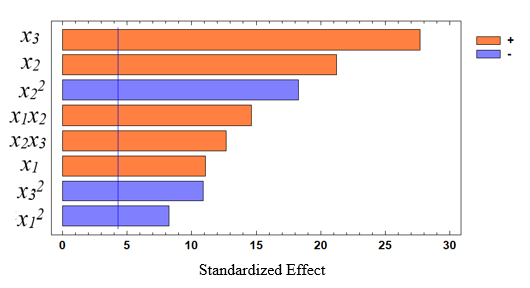
\includegraphics[width=0.6\textwidth]{media/pish2/image81}
	\caption*{Fig.1 - Pareto Chart of Standardized Effects of Independent Factors on the Viscosity of the Curd Product}
\end{figure}

\begin{figure}[H]
	\centering
	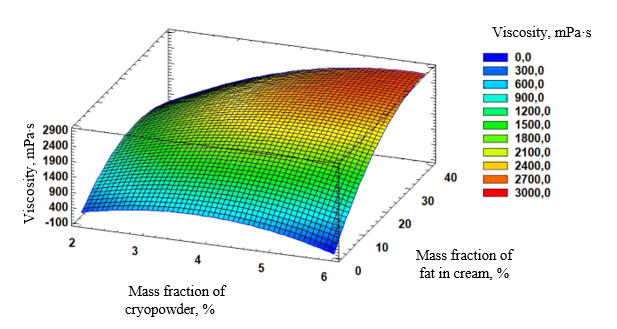
\includegraphics[width=0.65\textwidth]{media/pish2/image82}
	\caption*{Fig.2 - Response surface of the dependence of curd product viscosity on the mass fraction of cryopowder and fat content in cream}
\end{figure}

\begin{multicols}{2}
The analysis of the Pareto chart shows the greatest contribution to the
viscosity of the curd product from the mass fractions of cryopowder and
fat in the cream {[}11{]}.

Refining the effects of independent factors can be achieved by analyzing
the response surfaces, which are 3D graphs of dependencies shown in
figures 2-4. These graphs describe the influence of the mass fractions
of dairy bases, cryopowders, and the fat content in the cream on the
structural-mechanical properties of the model systems, and the response
surfaces characterize the patterns of structure formation in products
with cryopowders.
\end{multicols}

\begin{figure}[H]
	\centering
	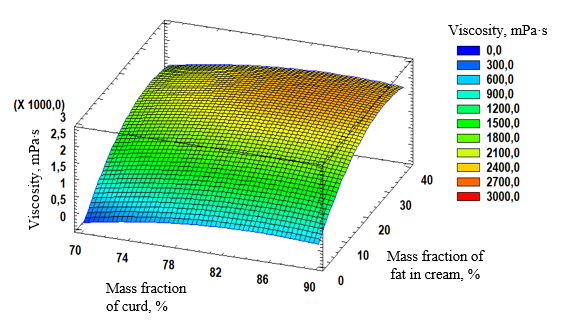
\includegraphics[width=0.65\textwidth]{media/pish2/image83}
	\caption*{Fig.3 - Response surface of the dependence of curd product
viscosity on the mass fraction of curd and fat content in cream}
\end{figure}

\begin{figure}[H]
	\centering
	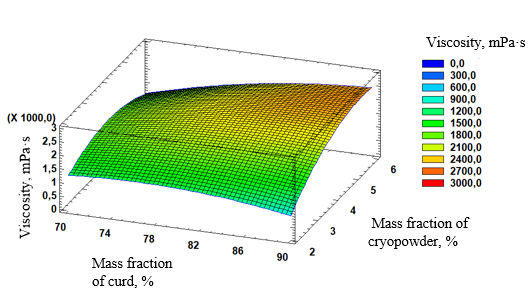
\includegraphics[width=0.65\textwidth]{media/pish2/image84}
	\caption*{Fig.4 - Response surface of the dependence of curd product viscosity on the mass fraction of curd and cryopowder}
\end{figure}

\begin{figure}[H]
	\centering
	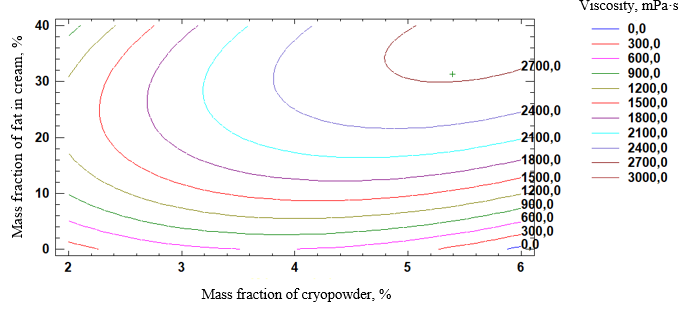
\includegraphics[width=0.65\textwidth]{media/pish2/image85}
	\caption*{Fig.5 - Sectional projections of the response surface illustrating the dependence of curd product viscosity on the mass fraction of cryopowder and fat content in cream}
\end{figure}

\begin{multicols}{2}
As seen in figures 2-4, the construction of the response surface for the
dependence of curd product viscosity on the mass fraction of curd and
cryopowder must take into account that these two components influence
the physicochemical properties of the mixture, including viscosity. The
optimal ranges of curd product viscosity were established as follows:
curd mass fraction - 89.6\%, cryopowder mass fraction - 5.4\%, and fat
content in cream - 31.3\%.

Figures 5-8 show sectional projections of the response surfaces
illustrating the dependence of curd product viscosity on the mass
fractions of cryopowder and fat in cream, which are key quality
indicators of the final product.
\end{multicols}

\begin{figure}[H]
	\centering
	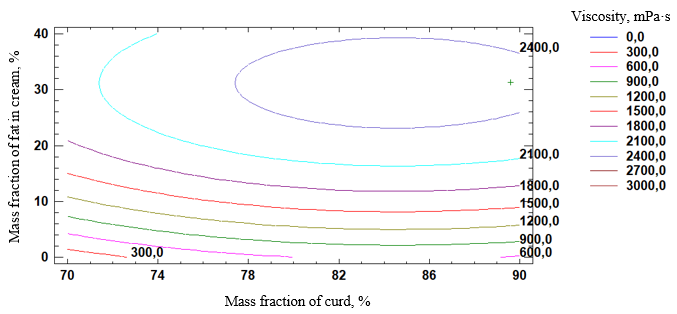
\includegraphics[width=0.7\textwidth]{media/pish2/image86}
	\caption*{Fig.6 - Sectional projections of the response surface illustrating the dependence of curd product viscosity on the mass fraction of curd and fat content in cream}
\end{figure}

\begin{figure}[H]
	\centering
	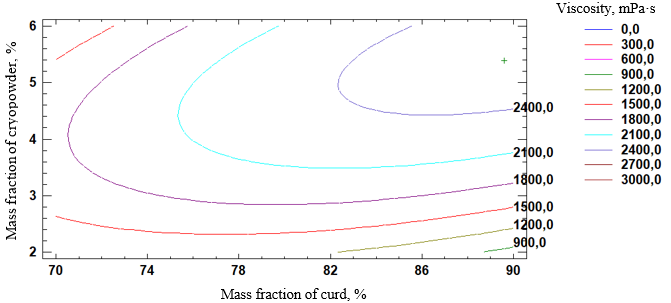
\includegraphics[width=0.7\textwidth]{media/pish2/image87}
	\caption*{Fig.7 - Sectional projections of the response surface
illustrating the dependence of curd product viscosity on the mass
fraction of curd and cryopowder}
\end{figure}

\begin{multicols}{2}
The analysis of the response surface behavior demonstrated that the
optimal viscosity range of the curd product is achieved at a curd
content of 89.6\%, cryopowder content of 5.4\%, and cream fat content of
31.3\%. The study of the error distribution in viscosity prediction
showed that a significant number of points remained close to the line,
indicating the accuracy of the developed model. Thus, the obtained
results make it possible to determine the optimal formulation parameters
of the curd product with the addition of cryopowder based on the
developed mathematical model.
\end{multicols}

\begin{figure}[H]
	\centering
	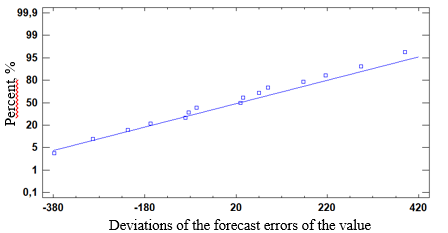
\includegraphics[width=0.7\textwidth]{media/pish2/image88}
	\caption*{Fig.8 - Diagnostic plot of deviation of predicted viscosity
error values from normal distribution}
\end{figure}

\begin{multicols}{2}
{\bfseries Conclusion.} Summarizing the obtained data, the following
conclusions can be drawn regarding the impact of the added cryopowders
on the curd product:

-on taste, color, and aroma: The amount of cryopowder introduced into
the dairy base affects the taste, color, and aroma of the curd product,
implying the presence of dosage limitations for cryopowder addition;

-on the content of functional food ingredients: The amount of functional
ingredients in the final product directly depends on the amount of added
cryopowder;

-on viscosity: The addition of pumpkin cryopowders within the studied
ranges provides the sample with a characteristic viscosity (for curd
products - 1400-2500 mPa·s) and consistency. Within the studied
concentration limits, cryopowders do not distort the product, making it
possible and easy to vary their content to ensure the desired high
flavor and color characteristics.

The above conclusions highlight the potential of using cryopowders in
dairy production as a versatile solution for creating natural products
with high nutritional and biological value. This approach also ensures
compliance with established standards and target product
characteristics, while enabling effective control over these parameters.
By adjusting formulation variables such as the mass fractions of the
dairy base, cryopowders, and cream (including their fat content), key
quality indicators of the final product---such as nutritional value,
content of functional ingredients, viscosity, and sensory
properties---can be efficiently managed.

\emph{{\bfseries Funding.} This research has funded by the Ministry of
Agriculture of the Republic of Kazakhstan (BR22886613).}
\end{multicols}

\begin{center}
{\bfseries References}
\end{center}

\begin{references}
1. Amit S.K. A review on mechanisms and commercial aspects of food
preservation and processing // Agric \& Food Secur. - 2017. - 6(51)- P.
1-22. DOI 10.1186/s40066-017-0130-8.

2. Thapa N. Functionality and therapeutic values of fermented foods //
Health benefits of fermented foods and beverages. - 2015. - Р.111-168.
DOI 10.1201/b18279-3.

3. Bagchi D. Nutraceutical and Functional Food Regulations in the United
States and Around the World.2nd Edition. -- Academic Press. - 2014. -
592 p. DOI10.1016/B978-0-12-373901-8.X0001-7.

4. Yankovskaya V. Food quality management based on qualimetric methods
// Proceedings of the 9th International Scientific Conference Rural
Development 2019, edited by prof. Asta Raupelienė, Kaunas, Lithuania:
Vytautas Magnus University. - 2019. - P.93-97. DOI
10.15544/RD.2019.005.

5. Izzo L. Target analysis and retrospective screening of mycotoxins and
pharmacologically active substan\-ces in milk using an
ultra-high-performance liquid chromatography/ high-resolution mass
spectrometry approach// J. Dairy Sci. - 2020. - Vol.103. - P.1250-1260.
DOI 10.3168/jds.2019-17277.

6. Preedy V.R. Handbook of food fortification and health // From
Concepts to Public Health Applications. - 2013. - 2013 р. DOI
10.1007/978-1-4614-7110-3.

7. Kamioka H. Quality of systematic reviews of the foods with function
claims in Japan: comparative before- and after-evaluation of
verification reports by the consumer affairs agency // Nutrients. -
2019. - Vol.11. - 19 p. DOI 10.3390/nu11071583.

8. Kirechev D. Risk Management Mechanisms in Agricultural Holdings in
Bulgaria.Fourth International Scientific Business Conference LIMEN. -
2018. - 597-602. DOI 10.31410/limen.2018.597.

9. Puvanenthiran A. Synergistic effect of milk solids and carrot cell
wall particles on the rheology and texture of yoghurt gels. - 2014. - №
62. - P.701-708. DOI 10.1016/j.foodres.2014.04.023.

10. Martirosyan D.M. A new definition of functional food by FFC: what
makes a new definition unique? // Functional foods in health and
disease. - 2015. - № 5(6). - P.209-223. DOI10.31989/ffhd.v5i6.183.

11. Prosekov A.Yu. The methodology of food design. Part 2. Digital
nutritiology in personal food // Theory and Practice of Meat Processing.
- 2021. - V.6. - № 4. - Р.328-334. DOI
10.21323/2414-438X-2021-6-4-328-334.
\end{references}

\begin{authorinfo}
\emph{{\bfseries Information about the authors}}

Alzhaxina N. - PhD, Director of the Astana branch of «Kazakh Research
Institute of Processing and Food Industry», Astana, Kazakhstan; e-mail:
\href{mailto:alzhaxina@inbox.ru}{\nolinkurl{alzhaxina@inbox.ru}};

Dalabayev A. - Master of Engineering and Technology, Senior Researcher
of the Astana branch of «Kazakh Research Institute of Processing and
Food Industry», Astana, Kazakhstan; e-mail: dalabaev\_askhat@mail.ru;

Aubakirova I. - Master' s student, Junior researcher,
Astana branch of «Kazakh Research Institute of Processing and Food
Industry», Astana, Kazakhstan; е-mail: aubakirova.inkar@bk.ru;

Mantay M. - bachelor, Junior researcher, Astana branch of «Kazakh
Research Institute of Processing and Food Industry», Astana, Kazakhstan;
е-mail:
\href{mailto:mako.mantay@mail.ru}{\nolinkurl{mako.mantay@mail.ru}}.

\emph{{\bfseries Сведения об авторах}}

Альжаксина Н.E. - PhD, и.о. директора Астанинского филиала ТОО
«Казахский научно-исследовательский институт перерабатывающей и пищевой
промышленности», Астана, Казахстан, е-mail:
\href{mailto:alzhaxina@inbox.ru}{\nolinkurl{alzhaxina@inbox.ru}};

Далабаев А.Б. - магистр техники и технологии, старший научный
сотрудник~Астанинского филиала ТОО «Казахский научно-исследовательский
институт перерабатывающей и пищевой промышленности», Астана, Казахстан,
е-mail: \\dalabaev\_askhat@mail.ru;

Аубакирова И.Е. - магистрант, младший научный сотрудник Астанинского
филиала ТОО «Казахский научно-исследоват\-ельский институт
перерабатывающей и пищевой промышленности», Астана, Казахстан, е-mail:
aubakirova.inkar@bk.ru;

Мантай М.С. - бакалавр, младший научный сотрудник Астанинского филиала
ТОО «Казахский научно-исследователь\-ский институт перерабатывающей и
пищевой промышленности», Астана, Казахстан, е-mail: mako.mantay@mail.ru~
\end{authorinfo}
